\section{Introduction}
\label{se:introduction}

In the second generation of intact stability criteria, the IMO addressed the importance of ships having sufficient roll damping to avoid large roll motions, parametric rolling, and excessive acceleration \parencite{imo_finalization_2016}. These phenomena have been well known for a very long time. Parametric roll was observed already by \parencite{froude_rolling_1861} and has been on the agenda of the marine research community since the early 1950s \parencite{galeazzi_early_2013}; it has received much more attention since \parencite{france_investigation_2001} showed that the APL China casualty in 1998, where a post-Panamax C11 class container ship lost almost a third of its containers, was most likely caused by head sea parametric rolling. The damping of roll motion plays an important part during the above-mentioned phenomena, and  \parencite{soder_ikeda_2019} showed that the relatively small difference in the roll damping prediction they obtained with small method variation, could mean the difference between severe roll angles and hardly noticeable motions. Experimental model tests are a widely accepted method to estimate a ship’s roll damping since the scale effect of the damping is mainly associated with the skin friction on ship hulls, and this friction contributes very little to a full-scale ship’s total roll damping \parencite{imo_1200_2006}. With the rapid increase in computation capability, computational fluid dynamics (CFD) methods have also been used to calculate roll damping, as in  \parencite{kristiansen_experimental_2014} and \parencite{henry_peter_piehl_ship_2016}. However, in the early stage of ship design, sometimes neither CFD methods nor experimental model tests are attractive options. For instance, when only limited information is available, such as the ship’s principal dimensions and the basic hull geometry, using CFD or model tests does not make sense. Also, when doing many design iterations, CFD or model tests can be too expensive and time consuming. Therefore, simpler methods are widely used in these cases. Several semi-empirical methods were proposed in the late 1970s \parencite{himeno_prediction_1981}. The most recognized method was developed in a series of research articles \parencite{ikeda_roll_1978,ikeda_eddy_1978,ikeda_roll_1979,ikeda_components_1978,ikeda_velocity_1979}, often referred to as Ikeda’s method and based on strip theory-analysis. This semi-empirical method is also recommended by \parencite{ittc_ittc_2011}. There also exists a newer and simplified version of Ikeda’s method \parencite{kawahara_simple_2011}  (named the SI-method here) where, unlike in Ikeda’s original method, strip-theory calculations are not needed, which makes it much easier to use in the design stages of ships. This method was developed as a regression on calculation results from Ikeda’s method for a series of parameterized hull shapes and is claimed \parencite{kawahara_simple_2011} to have almost the same accuracy as the original method within its limits. Ship designs have, however, evolved since the 1970s when Ikeda’s method was developed. So, the authors of the present paper wanted to see if these methods are still valid for newer ship geometries. The main objective of this paper is therefore to investigate the accuracy of the SI-method (being the newer and simplified version of Ikeda’s method) using a database of more than 250 roll decay model tests. The ships from these tests are recognized as being representative of modern merchant ships that have been tested at SSPA during the past 15 years, including, for instance, oil tankers, LNG tankers, passenger ships, car carriers, and others. Furthermore, possible ways to improve the accuracy of the SI-method for these ships will be investigated.

To make the paper complete, the conducted work according to Fig.\ref{fig:workflow} is divided in Section \ref{se:methods_for_prediction_and_analysis}, which presents the basic governing equations of roll motions and how roll damping can be obtained from roll decay tests and the SI-method. Based on the roll decay test database, different methods to estimate roll damping are compared in Section \ref{se:accuracy_SI_method}. Section \ref{se:correction_SI_method} proposes two new regression-based methods to improve the accuracy of roll damping in comparison to the SI-method. Conclusions are given in Section \ref{se:conclusions}.
 

\begin{figure}[H]
    \centering
    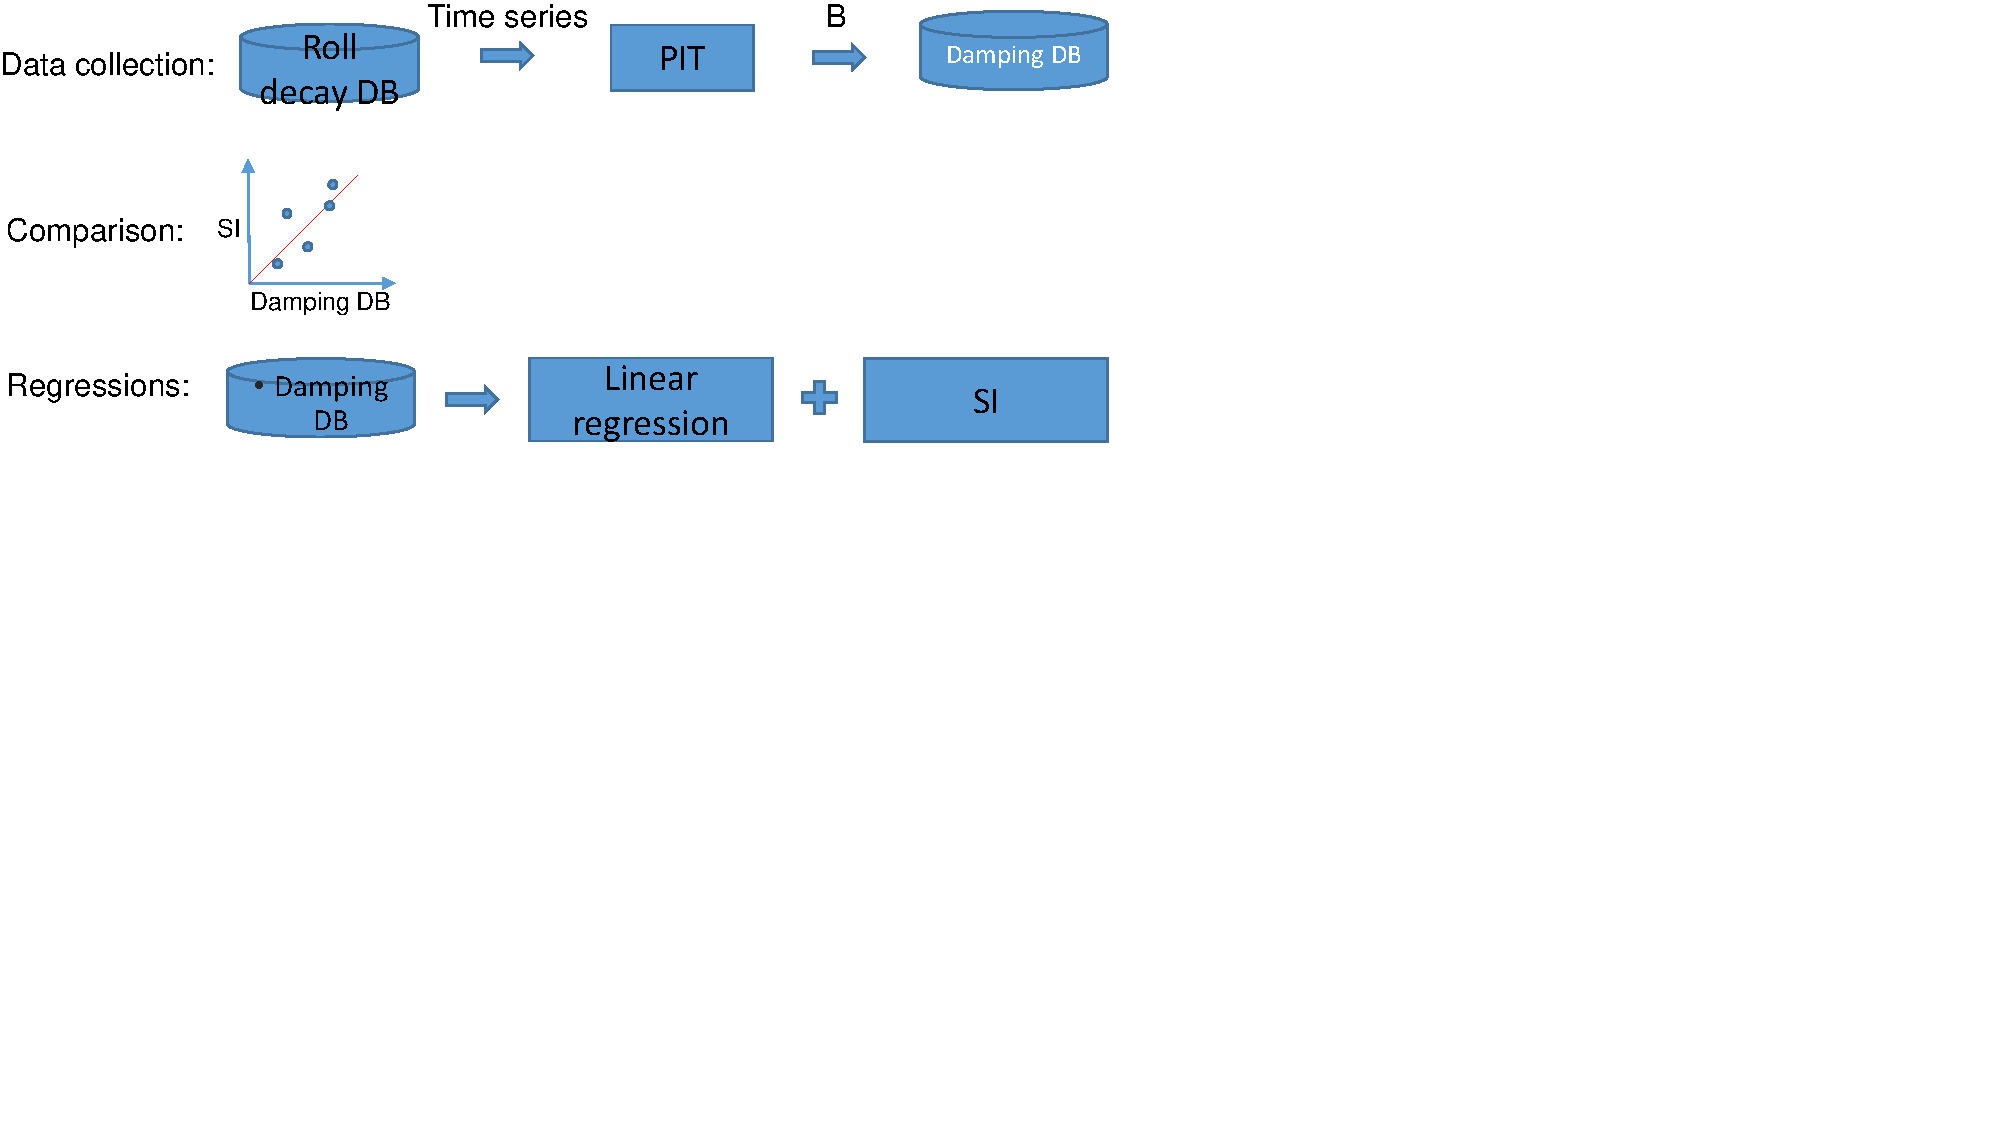
\includegraphics[width=0.5\columnwidth]{figures/workflow.pdf}
    \caption{Overview of the work conducted for this paper.}
    \label{fig:workflow}
\end{figure}